\usepackage[letterpaper,margin=15mm,top=18mm,bottom=18mm,headheight=15pt,headsep=5mm,footskip=10mm]{geometry}
\usepackage[T1]{fontenc}
\usepackage{helvet}
\renewcommand{\familydefault}{\sfdefault}
\usepackage{tikz}
\usetikzlibrary{arrows.meta,calc}
\usepackage{fancyhdr}
\usepackage{array}
\usepackage{xcolor}
\definecolor{redgood}{RGB}{185,63,68}
\definecolor{bluegood}{RGB}{41,107,164}
\definecolor{pale}{RGB}{243,244,245}
\definecolor{ink}{RGB}{30,35,40}
\color{ink}
\setlength{\parindent}{0pt}
\setlength{\parskip}{3.5mm}
\renewenvironment{center}{\par\vspace{1mm}\centering}{\par\vspace{1mm}}
\pagestyle{fancy}
\fancyhf{}
\renewcommand{\headrulewidth}{0pt}
\renewcommand{\footrulewidth}{0pt}
\fancyhead[L]{\small Week 58 / Fair division / \Band}
\fancyfoot[L]{\scriptsize Bellingham Math Circle / Week 58 / W58-\Packet-v2}
\fancyfoot[R]{\scriptsize\thepage}
\newcommand{\Band}{Grades 2--5}
\newcommand{\Packet}{shared}
\newcommand{\newband}[1]{\newpage\renewcommand{\Band}{#1}}
\newcommand{\prob}[2]{\noindent\textbf{Problem #1:} #2\par}
\newcommand{\good}[4]{% x y type label, in mm
  \ifnum#3=1\def\gc{redgood}\fi
  \ifnum#3=2\def\gc{bluegood}\fi
  \draw[rounded corners=1mm,fill=white,draw=ink,line width=.6pt] (#1,#2) rectangle ++(25,25);
  \ifnum#3=1\draw[fill=\gc,draw=\gc] (#1+12.5,#2+15.5) circle (4.2mm);\fi
  \ifnum#3=2\draw[fill=\gc,draw=\gc] (#1+8.3,#2+11.3) rectangle ++(8.4,8.4);\fi
  \node[font=\small] at (#1+12.5,#2+5) {#4};
}
\newcommand{\smallgood}[4]{% x y type label, mm
  \ifnum#3=1\def\gc{redgood}\fi
  \ifnum#3=2\def\gc{bluegood}\fi
  \draw[rounded corners=.8mm,fill=white,draw=ink,line width=.5pt] (#1,#2) rectangle ++(14,17);
  \ifnum#3=1\draw[fill=\gc,draw=\gc] (#1+7,#2+11) circle (2.6mm);\fi
  \ifnum#3=2\draw[fill=\gc,draw=\gc] (#1+4.4,#2+8.4) rectangle ++(5.2,5.2);\fi
  \node[font=\scriptsize] at (#1+7,#2+3) {#4};
}
\newcommand{\valuedots}[3]{% x y count
  \ifnum#3>0\foreach \i in {1,...,#3}{\fill[ink] (#1+4*\i,#2) circle (1.1mm);}\fi
}
\newcommand{\linearea}[1]{\vspace{1mm}\foreach \i in {1,...,#1}{\noindent\rule{\linewidth}{.25pt}\par\vspace{8mm}}}
\newcommand{\trayrecord}[2]{% x y
  \draw[rounded corners=2mm,draw=black!45,line width=.7pt] (#1,#2) rectangle ++(82,26);
  \node[anchor=north west,font=\small] at (#1+3,#2+24){A};
  \draw[black!25] (#1+41,#2+2) -- (#1+41,#2+24);
  \node[anchor=north west,font=\small] at (#1+44,#2+24){B};
}
\newcommand{\prefmini}{
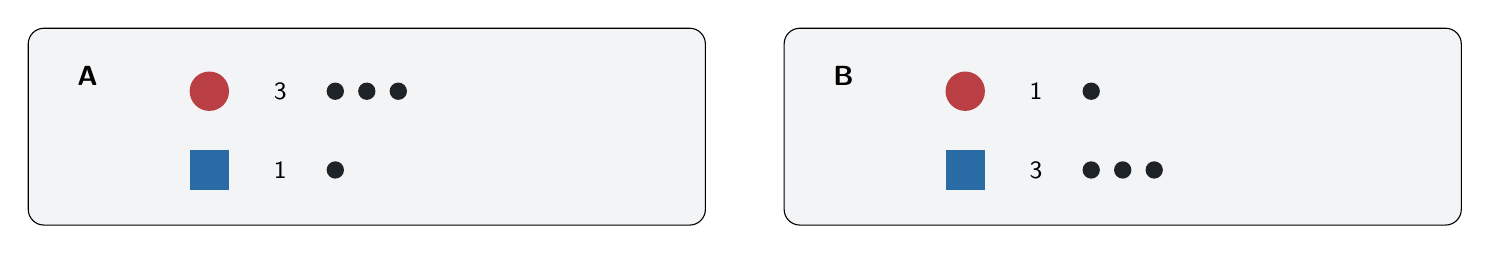
\begin{tikzpicture}[x=1mm,y=1mm]
  \foreach \x/\name/\r/\b in {0/A/3/1,96/B/1/3}{
    \draw[rounded corners=2mm,fill=pale] (\x,0) rectangle ++(86,25);
    \node[anchor=west,font=\bfseries] at (\x+5,19){\name};
    \fill[redgood] (\x+23,17) circle (2.5mm);
    \node[font=\small] at (\x+32,17){\r};
    \valuedots{\x+35}{17}{\r}
    \fill[bluegood] (\x+20.5,4.5) rectangle ++(5,5);
    \node[font=\small] at (\x+32,7){\b};
    \valuedots{\x+35}{7}{\b}
  }
\end{tikzpicture}}
\newcommand{\strip}[2]{% x y: schematic 180x24
  \draw[fill=redgood!22] (#1,#2) rectangle ++(90,24);
  \draw[fill=bluegood!22] (#1+90,#2) rectangle ++(90,24);
  \draw (#1,#2) rectangle ++(180,24);
  \draw (#1+90,#2) -- ++(0,24);
  \node[font=\small] at (#1+45,#2+12){red: 150 mm};
  \node[font=\small] at (#1+135,#2+12){blue: 150 mm};
}
\newcommand{\checkbar}[2]{
  \draw[line width=.8pt] (#1,#2) -- ++(100,0);
  \draw[line width=.8pt] (#1,#2-2) -- ++(0,4);
  \draw[line width=.8pt] (#1+100,#2-2) -- ++(0,4);
  \node[font=\small,anchor=south] at (#1+50,#2+2){100 mm};
}
